\documentclass[tikz, border=1mm]{standalone}

\usetikzlibrary{positioning}
\usepackage{xcolor}

\begin{document}
	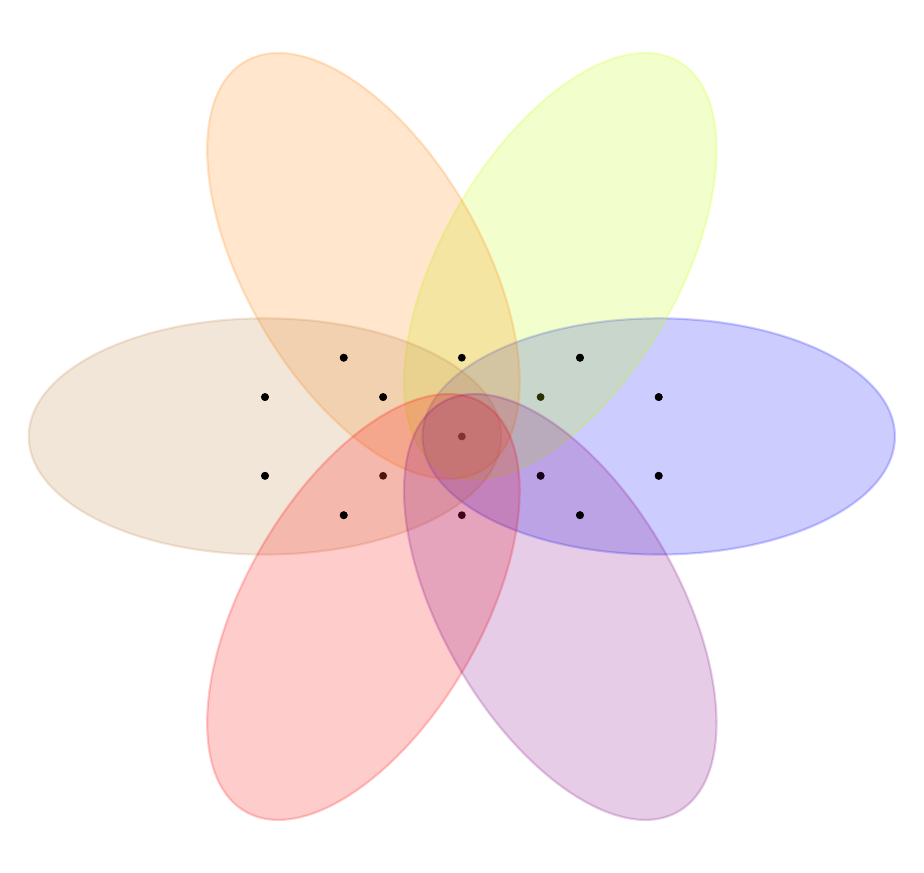
\begin{tikzpicture}
	\node[fill=black, circle, inner sep=1pt] (common) at (0,0) {};
	
	% First oval and points
	\draw[rotate=0, thick, blue, fill, opacity=0.2] (2.5,0) ellipse (3cm and 1.5cm);
	\node[fill=black, circle, inner sep=1pt] (p1) at (-1,0.5) {};
	\node[fill=black, circle, inner sep=1pt] (p2) at (1,0.5) {};
	\node[fill=black, circle, inner sep=1pt] (p3) at (-1,-0.5) {};
	\node[fill=black, circle, inner sep=1pt] (p4) at (1,-0.5) {};
	
	% Second oval and points
	\draw[rotate=60, thick, lime, fill, opacity=0.2] (2.5,0) ellipse (3cm and 1.5cm);
	\node[fill=black, circle, inner sep=1pt] (p5) at (1.5,1) {};
	\node[fill=black, circle, inner sep=1pt] (p6) at (-1.5,-1) {};
	\node[fill=black, circle, inner sep=1pt] (p7) at (2.5,0.5) {};
	\node[fill=black, circle, inner sep=1pt] (p8) at (-2.5,-0.5) {};
	
	% Third oval and points
	\draw[rotate=120, thick, orange, fill, opacity=0.2] (2.5,0) ellipse (3cm and 1.5cm);
	\node[fill=black, circle, inner sep=1pt] (p9) at (1.5,-1) {};
	\node[fill=black, circle, inner sep=1pt] (p10) at (-1.5,1) {};
	\node[fill=black, circle, inner sep=1pt] (p11) at (2.5,-0.5) {};
	\node[fill=black, circle, inner sep=1pt] (p12) at (-2.5,0.5) {};
	
	% Fourth oval and points
	\draw[rotate=180, thick, brown, fill, opacity=0.2] (2.5,0) ellipse (3cm and 1.5cm);
	\node[fill=black, circle, inner sep=1pt] (p13) at (-1,0.5) {};
	\node[fill=black, circle, inner sep=1pt] (p14) at (1,-0.5) {};
	\node[fill=black, circle, inner sep=1pt] (p15) at (0,-1) {};
	\node[fill=black, circle, inner sep=1pt] (p16) at (0,1) {};
	
	% Fifth oval and points
	\draw[rotate=240, thick, red, fill, opacity=0.2] (2.5,0) ellipse (3cm and 1.5cm);
	\node[fill=black, circle, inner sep=1pt] (p17) at (1.5,1) {};
	\node[fill=black, circle, inner sep=1pt] (p18) at (-1.5,-1) {};
	\node[fill=black, circle, inner sep=1pt] (p19) at (2.5,0.5) {};
	\node[fill=black, circle, inner sep=1pt] (p20) at (-2.5,-0.5) {};
	
	% Sixth oval and points
	\draw[rotate=300, thick, violet, fill, opacity=0.2] (2.5,0) ellipse (3cm and 1.5cm);
	\node[fill=black, circle, inner sep=1pt] (p21) at (1.5,-1) {};
	\node[fill=black, circle, inner sep=1pt] (p22) at (-1.5,1) {};
	\node[fill=black, circle, inner sep=1pt] (p23) at (2.5,-0.5) {};
	\node[fill=black, circle, inner sep=1pt] (p24) at (-2.5,0.5) {};
	
\end{tikzpicture}
\end{document}